\documentclass[11pt, a4paper]{article}
\sloppy %prevents text from going over the right margin
% \usepackage[T1]{fontenc}
\usepackage[utf8]{inputenc}
\usepackage{listings}
\usepackage[margin=1.0in]{geometry}
\usepackage{color}
\usepackage{graphicx}
\usepackage{tabularx}
\usepackage{url}
\usepackage[normalem]{ulem} 
\usepackage{enumitem}
\usepackage{hyperref}
\usepackage{fancyhdr} %Package to configure headings and footer
\usepackage{lastpage}
\usepackage{gensymb}
\usepackage[ngerman]{babel}
\setlength\parindent{0pt}

\newcommand{\VARtitle}{NW2}
\newcommand{\VARauthor}{Janeczek}

\title{Meteorologie \\ \VARtitle}
\author{\VARauthor}
\date{\today{}, Vienna}

% header
\pagestyle{fancy}
\fancyhead[L]{\today}
\fancyhead[R]{\VARtitle}

%footer
\fancyfoot[L]{\VARauthor}
\fancyfoot[C]{5AHITT}
\fancyfoot[R]{Page \thepage/\pageref{LastPage}}


\begin{document}

\lstset{ %
  backgroundcolor=\color{white},   % choose the background color; you must add \usepackage{color} or \usepackage{xcolor}
  basicstyle=\footnotesize,        % the size of the fonts that are used for the code
  breakatwhitespace=false,         % sets if automatic breaks should only happen at whitespace
  breaklines=true,                 % sets automatic line breaking
  captionpos=b,                    % sets the caption-position to bottom
% commentstyle=\color{mygreen},    % comment style
  deletekeywords={...},            % if you want to delete keywords from the given language
  escapeinside={\%*}{*)},          % if you want to add LaTeX within your code
  extendedchars=false,              % lets you use non-ASCII characters; for 8-bits encodings only, does not work with UTF-8
% frame=single,                    % adds a frame around the code
  keepspaces=true,                 % keeps spaces in text, useful for keeping indentation of code (possibly needs columns=flexible)
% keywordstyle=\color{blue},       % keyword style
% language=bash,                   % the language of the code
  morekeywords={*,...},            % if you want to add more keywords to the set
  numbers=left,                    % where to put the line-numbers; possible values are (none, left, right)
  numbersep=5pt,                   % how far the line-numbers are from the code
  rulecolor=\color{black},         % if not set, the frame-color may be changed on line-breaks within not-black text (e.g. comments (green here))
  showspaces=false,                % show spaces everywhere adding particular underscores; it overrides 'showstringspaces'
  showstringspaces=false,          % underline spaces within strings only
  showtabs=false,                  % show tabs within strings adding particular underscores
  stepnumber=1,                    % the step between two line-numbers. If it's 1, each line will be numbered
  tabsize=2,                       % sets default tabsize to 2 spaces
  title=\lstname                   % show the filename of files included with \lstinputlisting; also try caption instead of title
}


\maketitle
\newpage
\tableofcontents
\newpage


\section{Vorwort}

In diesem Dokument wird eine meiner naturwissenschaftlichen Thematiken ausgearbeitet. Es handelt sich um den Fachbereich der Meteorologie. Ich werde euch einen wesentlichen Überblick bezüglich der Inversionswetterlage, des Föhns sowie des Golfstroms liefern.

\section{Inversionswetterlage}

\subsection{Begriffserklärung}
\textbf{Was versteht man unter einer sogenannten Inversionswetterlage?}\\
Um näher auf die Inversionswetterlage eingehen zu können, muss der Begriff des \textit{Atmosphärischen Temperaturgradienten}\cite{atm-gradient} erklärt werden. Prinzipiell befindet sich der atmosphärische Temperaturgradient in der Erdatmosphäre und durch ihn wird beschrieben, wie sehr die Lufttemperatur mit der Höhe zu- oder abnimmt. \\

Durch die Umkehr dieses Temperaturgradienten (lateinisch: inversio), spricht man von einer Inversionswetterlage: Die oberen Luftschichten sind hierbei wärmer als die unteren. \\

In Folge steigt die Lufttemperatur mit der Höhe an, was die Schichtungsstabilität der Troposphäre und insbesondere alle kovektiven Prozesse beeinflusst. Der Bereich, in dem diese Inversion auftritt, wird als Inversionsschicht bezeichnet.\\

\subsection{Entstehung}
Ein Beispiel für eine Inversion lässt sich im Winter beobachten, wenn in klaren Nächsten der Boden auskühlen kann. Dieser kühlt somit auch die unterste Luftschicht, sodass diese stärker abkühlt, als die Luftschichten darüber. Am nächsten Morgen zeigt sich dann bis zur Grenze dieser Schicht der uns bekannte Bodennebel, da die Temperatur der bodennahen Schicht unter den Taupunkt fällt (jener Punkt an dem die relative Luftfeuchtigkeit 100 Prozent beträgt). \\

\begin{figure}[h!]
	\centering
	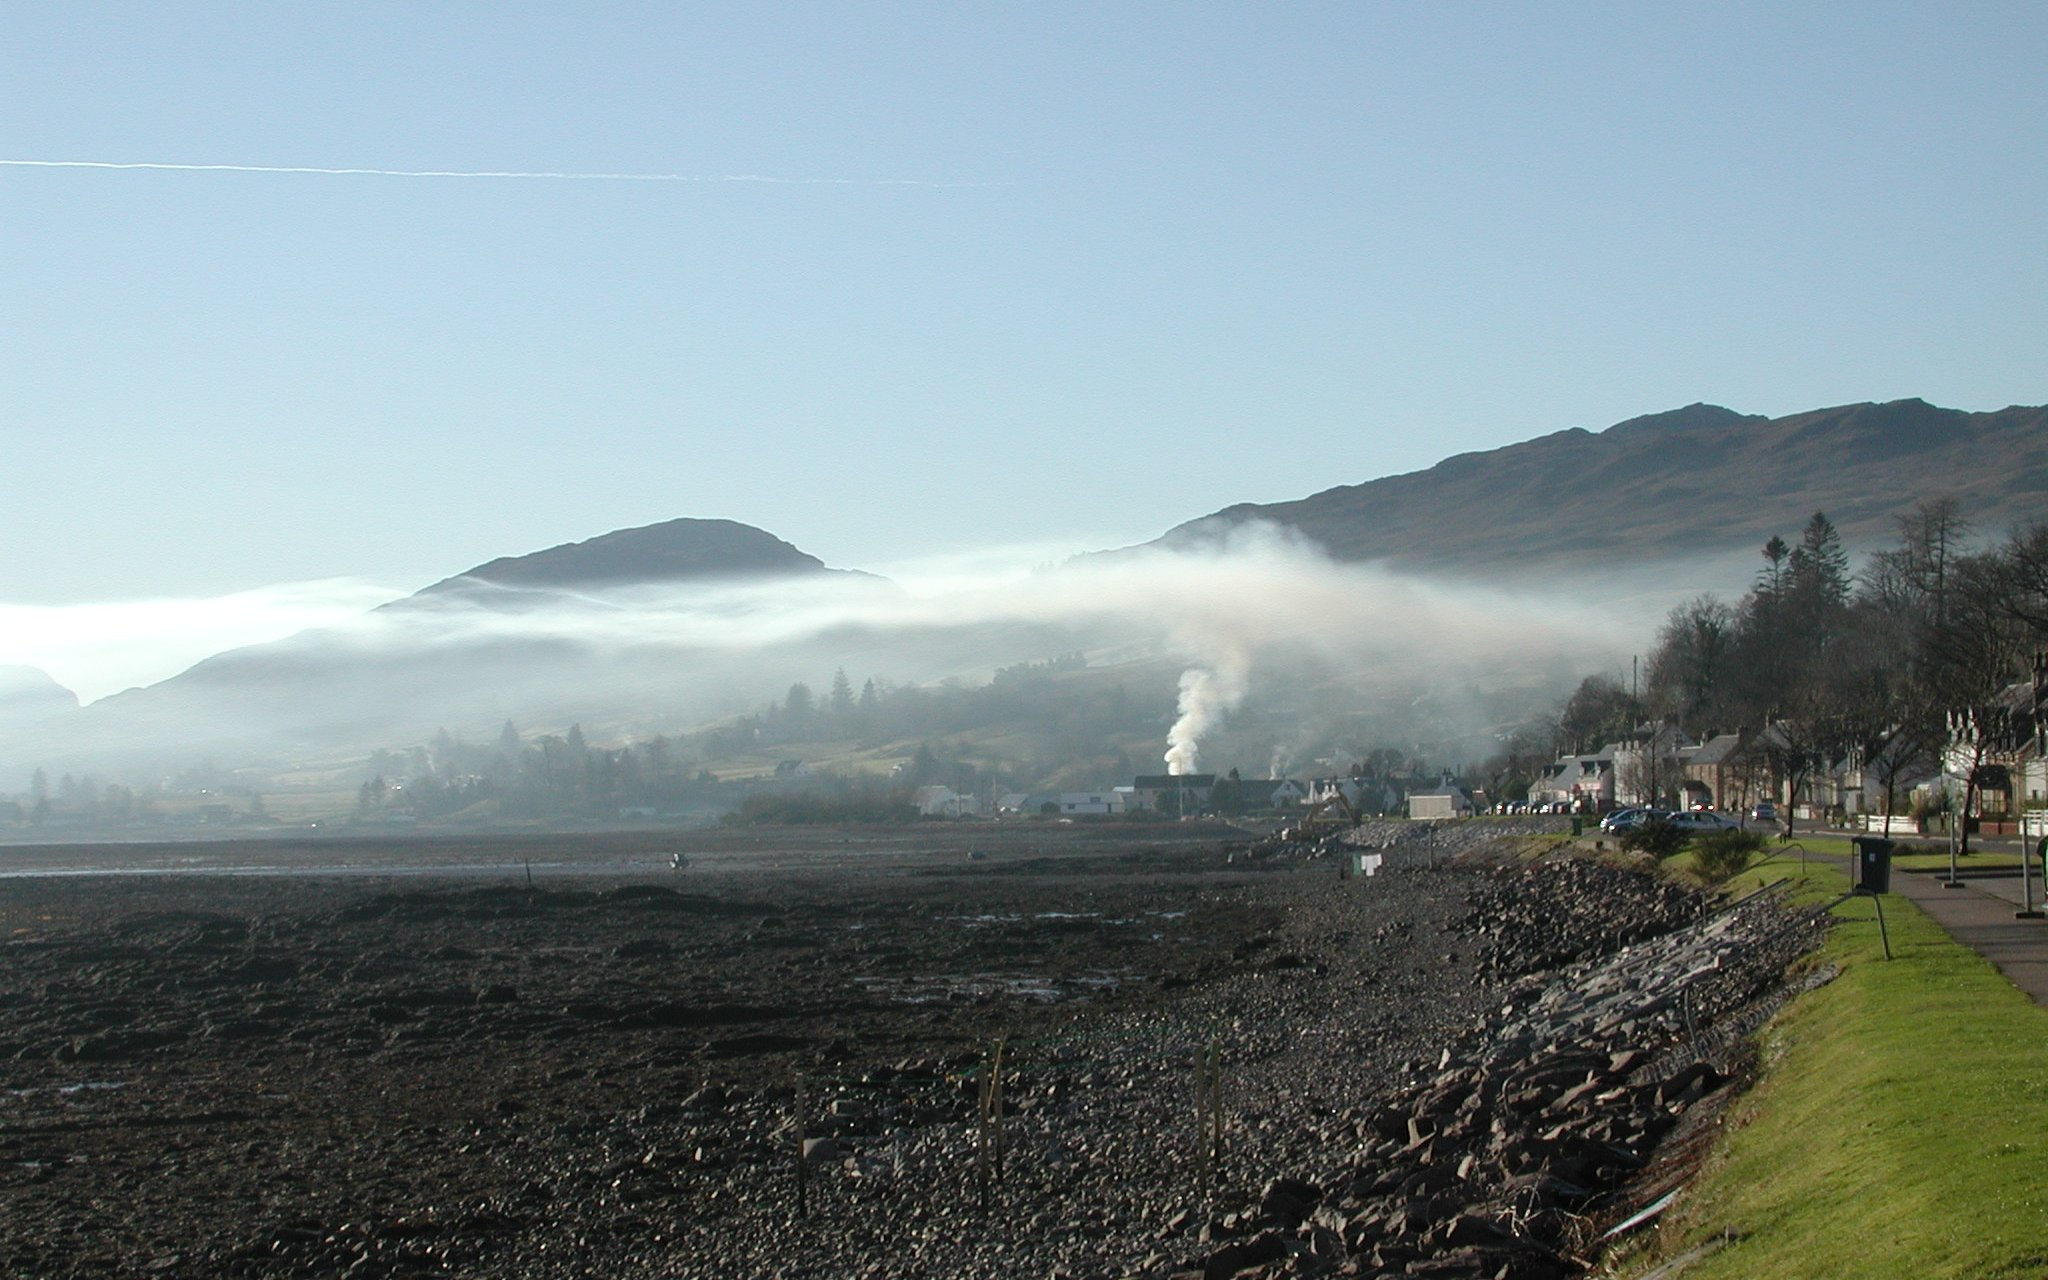
\includegraphics[width=0.7\textwidth]{images/inversio}
	\caption{Eine Inversionswetterlage in Lochcarron \cite{inversio-image}}
\end{figure}
\newpage
Aufgrund der höheren Dichte der kälteren Luftschicht, wird die Vermischung mit der darüber liegenden wärmeren Luftschift weitgehend unterdrückt. Die untere Schicht wird also von der oberen abgeschirmt, man spricht von einer stabilen Schichtung. Konvektive Prozesse, beziehungsweise Mechanismen zur Wärmeübertragung von thermischen Energien von einem Ort zu einem anderen, werden verhindert.\cite{inversion-klett}\cite{inv-wetterlage}\cite{entstehung-inverw} \\

\begin{figure}[h!]
	\centering
	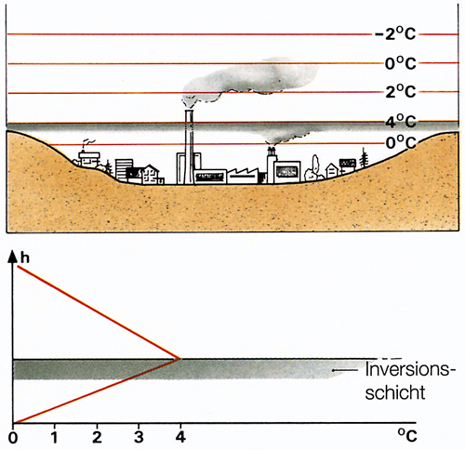
\includegraphics[width=0.7\textwidth]{images/inversion}
	\caption{Illustration einer Inversionswetterlage \cite{inversion-klett-image}}
\end{figure}
Ein aufsteigendes Luftpaket kühlt sich adiabatisch ab (ohne jeglichen Einfluss von anderen Wärmequellen, es findet kein Wärmeaustausch statt). Da in der Inversionsschicht wärmere Luft oberhalb von kälterer Luft liegt, ist das gerade aufgestiegene Luftpaket schon kälter als seine Umgebung und sinkt daher gleich wieder ab. Der eigentliche Luftaustausch bzw. eine Konvektion ist in der Inversionsschicht nicht möglich. \\

Inversionswetterlagen sorgen auch für geänderte Ausbreitungsbedingungen für Funkwellen. Diese werden am Dichteübergang ins dichtere Medium, hier die kalte Bodenluft totalreflektiert. Es wird gerne von diesem Effekt Gebrauch gemacht, um die Reichweite von Signalen zu erhöhen. Bei UKW (Ultrakurzwellen), die sich im Bereich von 30MHz - 300MHz befinden, kommt es sogar zu Überreichweiten. \\

\newpage
\subsection{Arten der Inversionswetterlage}
\subsubsection{Tropopause}
Nicht nur kann eine Inversionswetterlage durch kalte Nächte enstehen, sondern auch durch die Tropopause: \\ \\
Die Inversion wird hier durch die Tropopause (=die wichtigste Grenzfläche der Erdatmosphäre, die in 6 bis 18 Kilometer Höhe liegt)\cite{tropopause} gebildet und erklärt sich durch die langsam zunehmende Ozonkonzentration (10 bis 15 Kilometer). Das sich dort befindende Ozon absorbiert den UV-B-Teil der Sonneneinstrahlung, was zu einer Temperaturerhöhung entgegen dem Trend der Temperaturabnahme mit der Höhe führt.

\begin{figure}[h!]
	\centering
	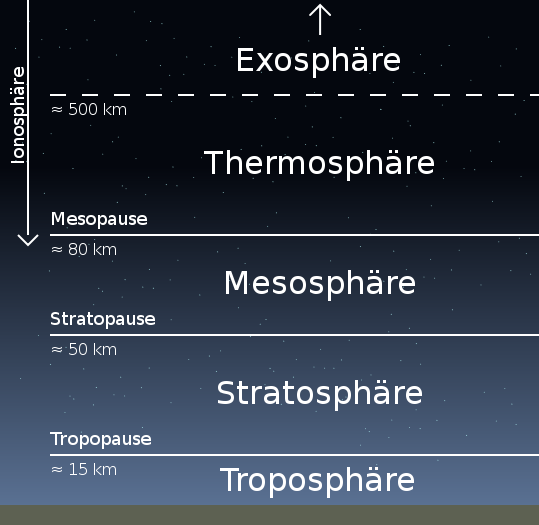
\includegraphics[width=0.5\textwidth]{images/tropo-image}
	\caption{Schichtung der Atmosphäre mit gekennzeichneter Troposphäre  \cite{tropo-image}}
\end{figure}

\subsubsection{Strahlungsinversion/Bodeninversion}
Wie bereits erwähnt nimmt die Lufttemperatur normalerweise mit steigender Höhe ab. Rauchgase aus Heizungsanlagen und Autoabgase führen (vor allem im Winter) zu erhöhten Staubkonzentrationen in der Luft. Staub filtert Sonnenlicht und wird dadurch erwärmt. \\ \\
Bei tagelanger Windstille steigt dieser Staub senkrecht auf und bildet eine warme, stabile Luftschicht, die über der unteren, kalten Luftschicht liegen bleibt ("Inversion").\\ \\
Abgase reichern sich in der Bodennähe und ergeben zusammen mit Bodennebel "dicke Luft", den uns bekannten Smog. Automotoren geben jedoch Wärme ab und können dazu beitragen bodennahe Luftschichten zu erwärmen.

\newpage
\section{Föhn}
\subsection{Begriffserklärung}
Der Föhn oder Föhnwind ist ein warmer, trockener Fallwind, der häufig auf der Leeseite von großen Gebirgen auftritt. \\ \\ Die Ausdrücke Luv und Lee wurden früher gerne von Seemännern verwendet, um die jeweilige Seite ihres Boots zu beschreiben. Die Luvseite ist die dem Wind zugewandte Seite und die Leeseite ist die dem Wind abgewandte Seite des Boots.
\subsection{Entstehung}
Der Föhn entsteht aus einer Windströmung über dem Gebirge, die mit Steigungsregen verbunden ist. Der Steigungsregen ist für die relativ warme Höhenluft verantwortlich. Er entsteht, wenn der Wind feuchte Luft vom Meer odeer Flachland an Gebirgszügen aufsteigen lässt. Prinzipiell handelt es sich hierbei um einen Wärmetransport, denn nachdem der Wind den Gebirgszug aufstiegen ist, muss dieser auf der anderen Seite fallen. \cite{foehn}\\

\begin{figure}[h!]
	\centering
	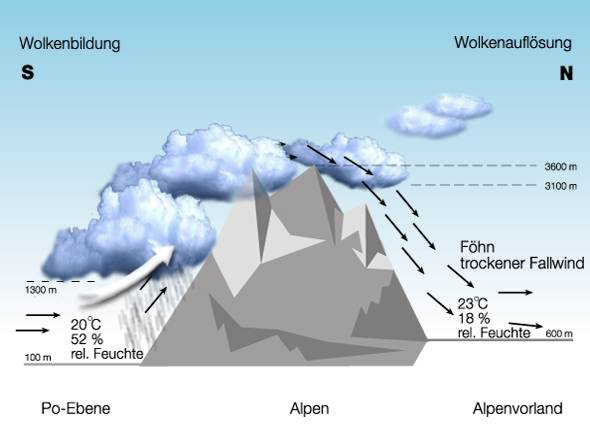
\includegraphics[width=0.7\textwidth]{images/foehn}
	\caption{Illustration des Föhnwindes \cite{foehn-image}}
\end{figure}

\noindent Fernsicht und gesundheitliche Beeschwerden, die von der erwärmten, trockenen, herabströmenden Luft verursacht werden sind aufgrund der aerosolarmen (=geringer Anteil an Schwebeteilchen in der Luft) Luftmassen. \\
Die Atmosphäre wird bei der Fernsicht auf zum Beispiel einen Berg wie ein Vergrößerungsglas. Wie schon gesagt nimmt die Dichte der Luft mit zunehmender Höhe ab, damit auch deren Brechungsindex. Das führt zu eeiner Ablenkung des Lichtes, Objekte erscheinen uns größer, näher. Dieser Effekt wird beim Föhn (zunehmende Temperatur, weitere Abnahme der Dichte) noch einmal verstärkt. \\

Außerdem gibt es die sogenannte Föhnkrankheit, da es bei Föhnwetterlagen zu vermehrten Auftreten von Herz- und Kreislaufproblemen kommt u.a. Kopfschmerzen und dergleichen.

\newpage
\section{Golfstrom}

Bei dem Golfstrom handelt es sich um eine rasch fließende Meeresströmung im Atlantik. In Richtung Europa fließt der sogenannte Nordatlantikstrom. Er ist Teil der wesentlichen Randströmung und beeinflusst das Klima in Nordeuropa. \\ \\
Der Golfstrom befördert $30*10^{6} $ Kubikmeter Wasser/Sekunde mit einer Geschwindigkeit von 18 m/s und bis zu maximal $15*10^{8}$ Kubikmeter Wasser/Sekunde bei dem 55$^{\circ}$ West. \\ \\
Dies entspricht über einem Hundertfachen an jener Menge Wasser, wie über alle Flüsse der Welt zusammen ins Meer fließt. Er transportiert ungefähr 15 Petawatt Leistung, das einer Nutzleistung von geschätzten 2 Millionen modernen Kraftwerken entspricht. \\ \\
Außerdem ist der Golfstrom Teil der globalen thermohalinen Zirkulation und ist als größte bekannte Wärmeströmung bekannt.

\begin{figure}[h!]
	\centering
	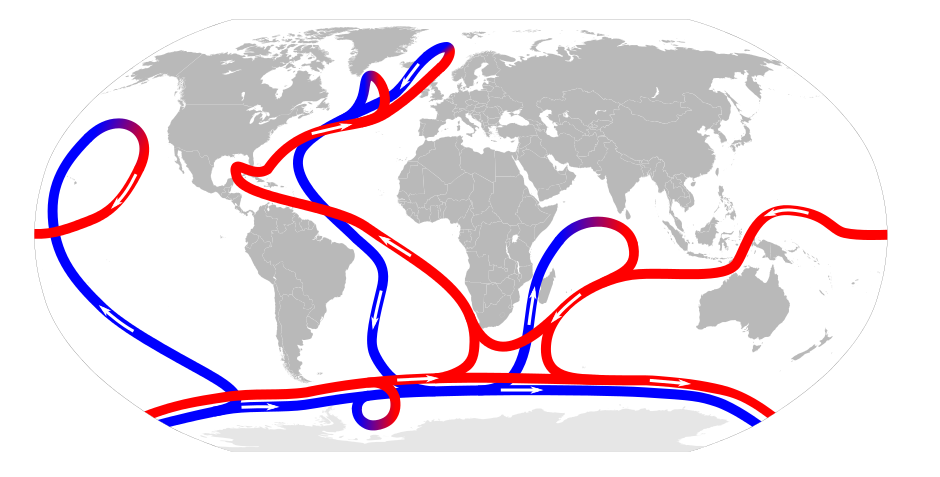
\includegraphics[width=0.9\textwidth]{images/thermo}
	\caption{Illustration der Thermohalinen Zirkulation \cite{thermo-image}}
\end{figure}

\begin{figure}[h!]
	\centering
	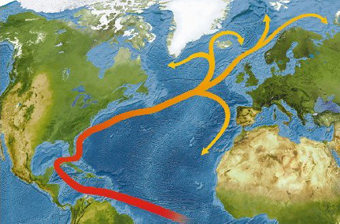
\includegraphics[width=0.6\textwidth]{images/golf}
	\caption{Illustration des Golfstroms mit sinkender Temperatur (rot zu gelb) \cite{golf-image}}
\end{figure}
\newpage
\nocite{*}
\bibliographystyle{plain}
\bibliography{bibliography}{}

\end{document}